\chapter{Results}
This chapter presents a description of the test sessions that were taken by anonymous test takers on the web platform. All the code for these results is presented can be found on GitHub\footnote{See the notebook in this repository \url{https://github.com/Oktogazh/analeksis}}. 

\section{Descriptive Statistics}
At time of writing, a total of 171 test sessions were collected. The average number of keys in each session was 47.743. As the number of distractors is expected to equal that of the keys, the average number of items per session was thus slighly less than a hundred. As a reminder, the length of the sessions depends on the score of the test takers. The higher a test taker is able to reach, the more real words it is allowed to keep seeing. The mean ratio of distractors recognised (false alarms) is 21.5\%, with an average of 9 pseudo-words recognised in absolute term. This last value seems surprisingly high and prompted further inquiry. Figure \ref{fig:score-fa} shows a distribution of the sessions final scores along with the ratio of recognised non-words.

As can be seen, even the highest scores had some cases of false alarms, and only a few low scores have a zero ratio. This means that the highest final score are also those sessions with the most cases of false alarms in absolute terms. Although somewhat unexpected, the fact that distractors are recognised from time to time by all ranges of scorers is encouraging. First, this means that the pseudo-words are well designed, validating the concept of using RNN for generating them. Also, the long-term trajectory of the distractors could also be stabilized by modifying the expectations before updating their rating in the back-end. By turning the chances of an item to be recognised to always be the false positive rate of the sessions (instead of the final rating like for the keys), the rating of most pseudo-words would stay in a range close to that of the pseudo-words. The poorly formed distractors would fall down in rating and the the non-nonsensical ones would rise up in a way where both would end up out of range. Note that this feature was not implemented yet, though it would be technically easy to do. The average range of false alarm is 207, that is, the difference between the highest and lowest ratings of the distractors recognised in a session. This is to put into perspective with the average score of 566. This means that false alarms started in average when the chance of recognising a real word are between 75\% and 50\%. So the chances of false alarms in this particular range when progression starts slowing down must be higher than the average of 21.5\% across the whole sessions. This point highlights the difficulty of modeling the tolerance to risk or potential cheating strategies. This could make the results non-comparable between different profiles, more on that in the next chapter.

A final, less surprising, observation, most sessions collected, 142, are from the Breton test. This is because the other tests were added to the platform at a later stage. Obviously, the Welsh, Ukrainian and French tests lack enough results for any serious analysis. This is the reason why we focus on the Breton test sessions in the following section.
\begin{figure}
    \centering
    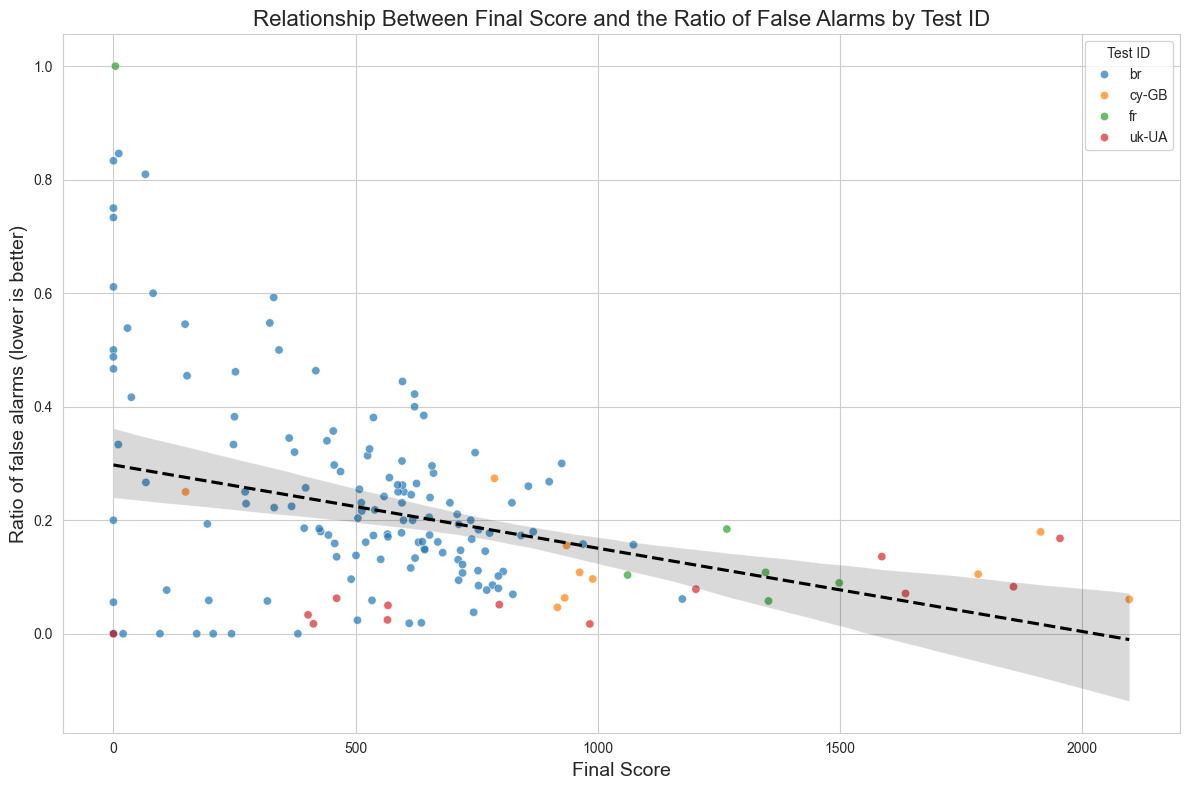
\includegraphics[width=0.8\linewidth]{figures/scores-fa.png}
    \caption{Distribution of the scores across several tests and their associated false positive rate}
    \medskip
    \small
\end{figure}\label{fig:score-fa}

\section{Measuring Adaptivity}
As mentioned in the previous chapter, we can use the last real-word recognition to test adaptivity. The number of last real words recognised in the last round of a Breton test is 73 out of 142, which makes 51.4\%. If we were trying to prove the hypothesis of faulty calibration of the system, we would need a p-value bellow 0.05. However, running a binomial test with these results yield a p-value of 0.801. This is really high, and does not invalidate the corresponding null hypothesis that the chances of recognising the last real word are highly uncertain. In other words, there is no reason to doubt in the precision and reliability of the test.

This result is highly encouraging in many ways. Firstly, only three categories of real words were used to pre-calibrate the items in the test. This means that the pre-calibration based long frequency lists is almost unnecessary which is valuable in a low-resource context. The benefits of using the modulo clustering technique to create an hybrid system between proportion of correct answers and a classic logistic scale is however comforted. Secondly, the level of precision claimed is really high. The precission is defined by the uncertainty function \ref{uncertainty-function}. It is variable, because dependant on the the number of real words seen in the session, number which depends on the length of the session, which depends on the rating progression. Unfortunately, the final value of the uncertainty function was not stored. It cannot be above ±52, if no word is recognised, and go down as the rating goes up.

As the early results on testing the adaptivity of the test were encouraging, we propose to extend the analysis to specific ranges. The result are given in the following table.

\begin{table}[h]
\centering
\begin{tabular}{|c|c|c|c|c|c|}
\hline
\textbf{ranges} & \textbf{sessions} & \textbf{recognised last word} & \textbf{observed mean} & \textbf{expected} & \textbf{p-value} \\
\hline
(0, 100] & 10 & 6 & 0.600000 & 0.5 & 0.753906 \\
(100, 200] & 7 & 1 & 0.142857 & 0.5 & 0.125000 \\
(200, 300] & 7 & 2 & 0.285714 & 0.5 & 0.453125 \\
(300, 400] & 12 & 6 & 0.500000 & 0.5 & 1.000000 \\
(400, 500] & 14 & 6 & 0.428571 & 0.5 & 0.790527 \\
(500, 600] & 29 & 16 & 0.551724 & 0.5 & 0.711071 \\
(600, 700] & 22 & 12 & 0.545455 & 0.5 & 0.831812 \\
(700, 800] & 22 & 13 & 0.590909 & 0.5 & 0.523467 \\
(800, 900] & 7 & 6 & 0.857143 & 0.5 & 0.125000 \\
(900, 1000] & 8 & 3 & 0.375000 & 0.5 & 0.726562 \\
(1000, 1100] & 2 & 1 & 0.500000 & 0.5 & 1.000000 \\
(1100, 1200] & 1 & 1 & 1.000000 & 0.5 & 1.000000 \\
(1200, 1300] & 2 & 0 & 0.000000 & 0.5 & 0.500000 \\
(1300, 1400] & 2 & 2 & 1.000000 & 0.5 & 0.500000 \\
(1400, 1500] & 1 & 0 & 0.000000 & 0.5 & 1.000000 \\
(1500, 1600] & 1 & 0 & 0.000000 & 0.5 & 1.000000 \\
(1600, 1700] & 1 & 0 & 0.000000 & 0.5 & 1.000000 \\
(1700, 1800] & 1 & 1 & 1.000000 & 0.5 & 1.000000 \\
(1800, 1900] & 1 & 0 & 0.000000 & 0.5 & 1.000000 \\
\hline
\end{tabular}
\caption{Recognition Rate of the Last Real Words by Score Ranges}
\label{tab:recognition_stats}
\end{table}

As can be seen, the low number of session for each range does not allow to unvalidate the idea that the last real word chance of being recognised are random. However, such hypothesis cannot be validated neither, we can only state that the result are so far consistant with it. Note that this method seem to be able to show early signs of potential ceiling effects. The transition from below to above 900 seems to show potential ceiling effects. The range 800–900 has a higher mean than 85\%, when the 900–1000 range drops to 37\%. Once again, the sample size is to small to confirm the presence of a significant ceiling effect. But this method of analysis could show such issues if a test is used at a larger scale. On the other hand, a wider adoption of the test would improve the calibration, and thus improve the results.